% begin module transformations-horizontal-stretches
\begin{frame}\ %
\uncover<1->{}
\psset{xunit=1.4cm, yunit=1.4cm}
\begin{pspicture}(-0.6, -1.4)(6.2,1.4)%
\tiny%
\fcAxesStandard{-0.6}{-1.4}{6.2}{1.4}%
%Function formula: sin{}(x)
\rput[b](1.57, 1.1){\alertNoH{1-2}{$y=f(x)$}}%
\newcommand{\theC}{1}%
\newcommand{\theFun}{x 57.29578 mul \theC\space mul sin\space}%
\uncover<1-2>{\psplot[linecolor=\fcColorGraph, plotpoints=1000]{-0.5}{6}{\theFun}}%
\uncover<3->{\psplot[linecolor=blue, plotpoints=1000]{-0.5}{6}{\theFun}}%
\newcommand{\curPt}{2}%
\newcommand{\theAni}[6]{%
\uncover<handout:0|####1>{\fcXTickWithLabel{\curPt\space}{$x$}}%
\uncover<handout:0|####2>{\fcXTickWithLabel{\curPt\space\theC\space mul}{$cx$}}%
\uncover<handout:0|####3>{\psline[linecolor=blue, linewidth=2pt](! \curPt\space\theC\space mul 0)(! \curPt\space\theC\space mul \curPt\space 1 dict begin /x exch def \theFun end)}%
\uncover<handout:0|####4>{\rput[l](! \curPt\space\theC\space mul \curPt\space 1 dict begin /x exch def \theFun end 2 div){$~~f(cx)$}}%
\uncover<handout:0|####5>{\psline[linecolor=red, linewidth=2pt](! \curPt\space 0)(! \curPt\space \curPt\space 1 dict begin /x exch def \theFun end)}%
\uncover<handout:0|####6>{\rput[l](! \curPt\space \curPt\space 1 dict begin /x exch def \theFun end 2 div){$~~f(cx)$}}%
}%
\renewcommand{\theC}{1.5}%
\renewcommand{\curPt}{1}%
\theAni{4-7}{5-7}{6-20}{6-7}{7-20}{7}%
\renewcommand{\curPt}{1.6}%
\theAni{8-11}{9-11}{10-20}{10-11}{11-20}{11}%
\renewcommand{\curPt}{2.2}%
\theAni{12-15}{13-15}{14-20}{14-15}{15-20}{15}%
\renewcommand{\curPt}{2.8}%
\theAni{16-19}{17-19}{18-20}{18-19}{19-20}{19}%
\uncover<handout:1|20-22>{%
\psplot[linecolor=\fcColorGraph, plotpoints=1000]{0 }{6}{\theFun}%
\rput[t](! 3.14  -1.1){\alertNoH{20-22}{$y=f(cx)$}}%
}%
\renewcommand{\theC}{0.5}
\uncover<handout:2|23->{%
\psplot[linecolor=\fcColorGraph, plotpoints=1000]{0 }{6}{\theFun}%
\rput[b](! 3.14 1.1){\alertNoH{23}{$y=f \left( \frac{x }{c}\right)$}}%
}%
\end{pspicture}
%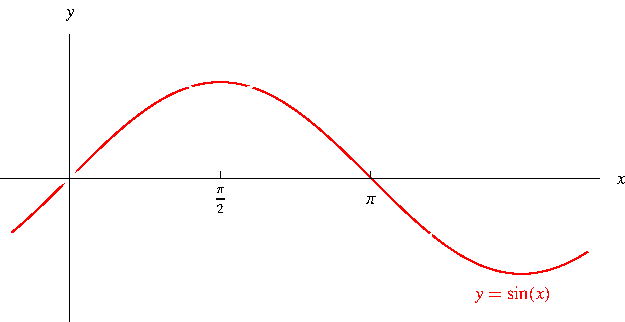
\includegraphics[height=6cm]{precalculus/pictures/01-03-stretcha.pdf}%
%}%
%\only<handout:0| 3>{%
%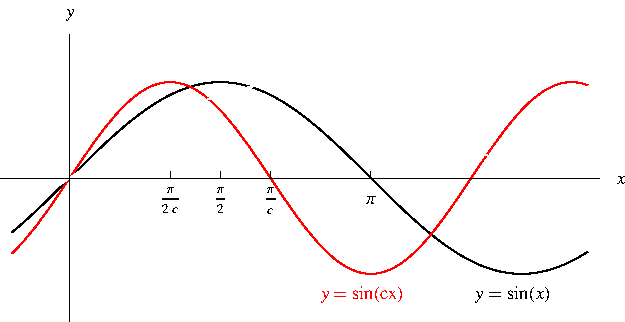
\includegraphics[height=6cm]{precalculus/pictures/01-03-stretchb.pdf}%
%}%
%\only<4->{%
%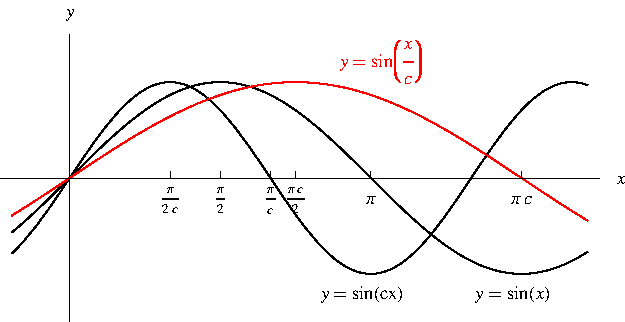
\includegraphics[height=6cm]{precalculus/pictures/01-03-stretchc.pdf}%
%}%a

\begin{itemize}
\item \alertNoH{3}{What happens if we multiply $x$ by const. $c > 1$ before applying $f$?}
\item \alertNoH{5}{What happens if we divide $x$ by const. $c > 1$ before applying $f$?}
\end{itemize}
\uncover<2->{
\begin{tabular}{|l|l|}
\hline
\alertNoH{ 3-22}{$f(cx)$} &%
\fcAnswerUncover{3}{22}{Compress the graph of $f(x)$ horizontally by a factor of $c$.} \\%
\alertNoH{ 4}{$f\left(\frac{1}{c}x\right)$} &%
\uncover<23->{\alertNoH{23}{Stretch the graph of $f(x)$ horizontally by a factor of $c$.}} \\%
\hline
\end{tabular}
}
\end{frame}
% end module transformations-horizontal-stretches
